\documentclass[border=10pt]{standalone}

\usepackage{tikz}
\usetikzlibrary{fit,positioning,calc}


%default strings
\providecommand{\tstrcommunication}{Communication\\ protocol}
\providecommand{\tstrobjects}{Objects}
\providecommand{\tstrucode}{Microcode}
\providecommand{\tstrhbusstack}{HBUS Stack}
\providecommand{\tstrhbusdevice}{HBUS Device}
\providecommand{\tstrdevicecode}{Device code (firmware)}

\begin{document}
\begin{tikzpicture}[auto]

\tikzstyle{stackitem}=[rounded corners,thick,rectangle,minimum height=50pt,minimum width=50pt,draw=black, node distance=20pt]

\node [stackitem,align=center] (comm) {\tstrcommunication};
\node [stackitem,right=20pt of comm] (obj) {\tstrobjects}; 
\node [stackitem,right=20pt of obj] (ucode) {\tstrucode};

\node [rounded corners,inner sep=10pt,draw=black,dashed,rectangle,fit= (comm) (obj) (ucode),label=120:{\tstrhbusstack}] (stack) {};

%calculate "stack" size
\path let \p1=($(stack.west)-(stack.east)$),
          \n1= {veclen(\p1)-0.4pt}
          in node [stackitem,above=52pt of stack.east ,align=center,anchor=south east,minimum width=\n1] (fw) {\tstrdevicecode};

%device
\node [dashed,rounded corners,thick,inner sep=10pt,draw=black,fit= (fw) (stack),label=120:{\tstrhbusdevice}] (device) {};
 
%bus
\node [draw=none,left = of comm.west,xshift=-10pt] (bus) {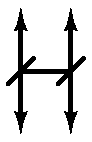
\includegraphics[scale=0.75]{hbuslogoh}}; 

\path [latex-latex,thick] (comm) edge (obj)
      [latex-latex,thick] (obj) edge (ucode)
      [latex-latex,thick] (fw) edge [out=270,in=90] (obj)
      [latex-latex,thick] (comm) edge (bus);

\end{tikzpicture}
\end{document}